% Options for packages loaded elsewhere
\PassOptionsToPackage{unicode,linktoc=all}{hyperref}
\PassOptionsToPackage{hyphens}{url}
\PassOptionsToPackage{dvipsnames,svgnames,x11names}{xcolor}
%
\documentclass[
  a4paper,
]{article}
\usepackage{amsmath,amssymb}
\usepackage{iftex}
\ifPDFTeX
  \usepackage[T1]{fontenc}
  \usepackage[utf8]{inputenc}
  \usepackage{textcomp} % provide euro and other symbols
\else % if luatex or xetex
  \usepackage{unicode-math} % this also loads fontspec
  \defaultfontfeatures{Scale=MatchLowercase}
  \defaultfontfeatures[\rmfamily]{Ligatures=TeX,Scale=1}
\fi
\usepackage{lmodern}
\ifPDFTeX\else
  % xetex/luatex font selection
\fi
% Use upquote if available, for straight quotes in verbatim environments
\IfFileExists{upquote.sty}{\usepackage{upquote}}{}
\IfFileExists{microtype.sty}{% use microtype if available
  \usepackage[]{microtype}
  \UseMicrotypeSet[protrusion]{basicmath} % disable protrusion for tt fonts
}{}
\makeatletter
\@ifundefined{KOMAClassName}{% if non-KOMA class
  \IfFileExists{parskip.sty}{%
    \usepackage{parskip}
  }{% else
    \setlength{\parindent}{0pt}
    \setlength{\parskip}{6pt plus 2pt minus 1pt}}
}{% if KOMA class
  \KOMAoptions{parskip=half}}
\makeatother
\usepackage{xcolor}
\usepackage[margin=25mm]{geometry}
\usepackage{longtable,booktabs,array}
\usepackage{calc} % for calculating minipage widths
% Correct order of tables after \paragraph or \subparagraph
\usepackage{etoolbox}
\makeatletter
\patchcmd\longtable{\par}{\if@noskipsec\mbox{}\fi\par}{}{}
\makeatother
% Allow footnotes in longtable head/foot
\IfFileExists{footnotehyper.sty}{\usepackage{footnotehyper}}{\usepackage{footnote}}
\makesavenoteenv{longtable}
\usepackage{graphicx}
\makeatletter
\def\maxwidth{\ifdim\Gin@nat@width>\linewidth\linewidth\else\Gin@nat@width\fi}
\def\maxheight{\ifdim\Gin@nat@height>\textheight\textheight\else\Gin@nat@height\fi}
\makeatother
% Scale images if necessary, so that they will not overflow the page
% margins by default, and it is still possible to overwrite the defaults
% using explicit options in \includegraphics[width, height, ...]{}
\setkeys{Gin}{width=\maxwidth,height=\maxheight,keepaspectratio}
% Set default figure placement to htbp
\makeatletter
\def\fps@figure{htbp}
\makeatother
\setlength{\emergencystretch}{3em} % prevent overfull lines
\providecommand{\tightlist}{%
  \setlength{\itemsep}{0pt}\setlength{\parskip}{0pt}}
\setcounter{secnumdepth}{-\maxdimen} % remove section numbering
\newlength{\cslhangindent}
\setlength{\cslhangindent}{1.5em}
\newlength{\csllabelwidth}
\setlength{\csllabelwidth}{3em}
\newlength{\cslentryspacingunit} % times entry-spacing
\setlength{\cslentryspacingunit}{\parskip}
\newenvironment{CSLReferences}[2] % #1 hanging-ident, #2 entry spacing
 {% don't indent paragraphs
  \setlength{\parindent}{0pt}
  % turn on hanging indent if param 1 is 1
  \ifodd #1
  \let\oldpar\par
  \def\par{\hangindent=\cslhangindent\oldpar}
  \fi
  % set entry spacing
  \setlength{\parskip}{#2\cslentryspacingunit}
 }%
 {}
\usepackage{calc}
\newcommand{\CSLBlock}[1]{#1\hfill\break}
\newcommand{\CSLLeftMargin}[1]{\parbox[t]{\csllabelwidth}{#1}}
\newcommand{\CSLRightInline}[1]{\parbox[t]{\linewidth - \csllabelwidth}{#1}\break}
\newcommand{\CSLIndent}[1]{\hspace{\cslhangindent}#1}
\ifLuaTeX
\usepackage[bidi=basic]{babel}
\else
\usepackage[bidi=default]{babel}
\fi
\babelprovide[main,import]{british}
% get rid of language-specific shorthands (see #6817):
\let\LanguageShortHands\languageshorthands
\def\languageshorthands#1{}
% $HOME/.pandoc/defaults/latex-header-includes.tex
% Common header includes for both lualatex and xelatex engines.
%
% Preliminaries
%
% \PassOptionsToPackage{rgb,dvipsnames,svgnames}{xcolor}
% \PassOptionsToPackage{main=british}{babel}
\PassOptionsToPackage{english}{selnolig}
\AtBeginEnvironment{quote}{\small}
\AtBeginEnvironment{quotation}{\small}
\AtBeginEnvironment{longtable}{\centering}
%
% Packages that are useful to include
%
\usepackage{graphicx}
\usepackage{subcaption}
\usepackage[inkscapeversion=1]{svg}
\usepackage[defaultlines=4,all]{nowidow}
\usepackage{etoolbox}
\usepackage{fontsize}
\usepackage{newunicodechar}
\usepackage{pdflscape}
\usepackage{fnpct}
\usepackage{parskip}
  \setlength{\parindent}{0pt}
\usepackage[style=american]{csquotes}
% \usepackage{setspace} Use the <fontname-plus.tex> files for setspace
%
\usepackage{esdiff} % for derivative symbols
\usepackage{amsmath}
\usepackage{hyperref} % cleveref must come AFTER hyperref
\usepackage[capitalize,noabbrev]{cleveref} % Must come after hyperref
% noto-plus.tex
% Font-setting header file for use with Pandoc Markdown
% to generate PDF via LuaLaTeX.
% The main font is Noto Serif.
% Other main fonts are also available in appropriately named file.
\usepackage{fontspec}
\usepackage{setspace}
\setstretch{1.3}
%
\defaultfontfeatures{Ligatures=TeX,Scale=MatchLowercase,Renderer=Node} % at the start always
%
% For English
% See also https://tex.stackexchange.com/questions/574047/lualatex-amsthm-polyglossia-charissil-error
% We use Node as Renderer for the Latin Font and Greek Font and HarfBuzz as renderer ofr Indic fonts.
%
\babelfont{rm}[Script=Latin,Scale=1]{NotoSerif}% Config is at $HOME/texmf/tex/latex/NotoSerif.fontspec
%
\babelfont{sf}[Script=Latin]{SourceSansPro}% Config is at $HOME/texmf/tex/latex/SourceSansPro.fontspec
%
\babelfont{tt}[Script=Latin]{FiraMono}% Config is at $HOME/texmf/tex/latex/FiraMono.fontspec
%
% Sanskrit, Tamil, and Greek fonts
%
\babelprovide[import, onchar=ids fonts]{sanskrit}
\babelprovide[import, onchar=ids fonts]{tamil}
\babelprovide[import, onchar=ids fonts]{greek}
%
\babelfont[sanskrit]{rm}[Scale=1.1,Renderer=HarfBuzz,Script=Devanagari]{NotoSerifDevanagari}
\babelfont[sanskrit]{sf}[Scale=1.1,Renderer=HarfBuzz,Script=Devanagari]{NotoSansDevanagari}
\babelfont[tamil]{rm}[Renderer=HarfBuzz,Script=Tamil]{NotoSerifTamil}
\babelfont[tamil]{sf}[Renderer=HarfBuzz,Script=Tamil]{NotoSansTamil}
\babelfont[greek]{rm}[Script=Greek]{GentiumBookPlus}
%
% Math font
%
\usepackage{unicode-math} % seems not to hurt % fallabck
\setmathfont[bold-style=TeX]{STIX Two Math}
%
%
% Other fonts
%
\newfontfamily{\emojifont}{Symbola}
%

\usepackage{titling}
\usepackage{fancyhdr}
    \pagestyle{fancy}
    \fancyhead{}
    \fancyfoot{}
    \renewcommand{\headrulewidth}{0.2pt}
    \renewcommand{\footrulewidth}{0.2pt}
    \fancyhead[LO,RE]{\scshape\thetitle}
    \fancyfoot[CO,CE]{\footnotesize Copyright © 2006\textendash\the\year, R (Chandra) Chandrasekhar}
    \fancyfoot[RE,RO]{\thepage}
\newfontfamily{\regulariconfont}{Font Awesome 6 Free Regular}[Color=Grey]
\newfontfamily{\solidiconfont}{Font Awesome 6 Free Solid}[Color=Grey]
\newfontfamily{\brandsiconfont}{Font Awesome 6 Brands}[Color=Grey]
%
% Direct input of Unicode code points
%
\newcommand{\faEnvelope}{\regulariconfont\ ^^^^f0e0\normalfont}
\newcommand{\faMobile}{\solidiconfont\ ^^^^f3cd\normalfont}
\newcommand{\faLinkedin}{\brandsiconfont\ ^^^^f0e1\normalfont}
\newcommand{\faGithub}{\brandsiconfont\ ^^^^f09b\normalfont}
\newcommand{\faAtom}{\solidiconfont\ ^^^^f5d2\normalfont}
\newcommand{\faPaperPlaneRegular}{\regulariconfont\ ^^^^f1d8\normalfont}
\newcommand{\faPaperPlaneSolid}{\solidiconfont\ ^^^^f1d8\normalfont}

%
% The block below is commented out because of Tofu glyphs in HTML
%
% \newcommand{\faEnvelope}{\regulariconfont\ \normalfont}
% \newcommand{\faMobile}{\solidiconfont\ \normalfont}
% \newcommand{\faLinkedin}{\brandsiconfont\ \normalfont}
% \newcommand{\faGithub}{\brandsiconfont\ \normalfont}
\ifLuaTeX
  \usepackage{selnolig}  % disable illegal ligatures
\fi
\IfFileExists{bookmark.sty}{\usepackage{bookmark}}{\usepackage{hyperref}}
\IfFileExists{xurl.sty}{\usepackage{xurl}}{} % add URL line breaks if available
\urlstyle{sf}
\hypersetup{
  pdftitle={The Two Most Important Numbers: Zero and One},
  pdfauthor={R (Chandra) Chandrasekhar},
  pdflang={en-GB},
  colorlinks=true,
  linkcolor={DarkOliveGreen},
  filecolor={Purple},
  citecolor={DarkKhaki},
  urlcolor={Maroon},
  pdfcreator={LaTeX via pandoc}}

\title{The Two Most Important Numbers: Zero and One}
\author{R (Chandra) Chandrasekhar}
\date{2023-10-31 | 2023-11-05}

\begin{document}
\maketitle

\thispagestyle{empty}


The unique properties of the numbers zero and one make them
mathematically interesting and indispensable. In this slow-paced stroll
though the ideas streaming out of these two numbers, we uncover
well-known as well as relatively obscure facts about them. It is hoped
that in the process we may discover how they cement together disparate
areas of Mathematics.

\hypertarget{starting-at-the-beginning}{%
\subsection{Starting at the beginning}\label{starting-at-the-beginning}}

At first, I thought I would skirt around the formal sets of numbers, and
concepts like commutativity and associativity, and keep this blog very
informal. But I found that each time I tried that approach, I would have
to furtively sneak in a paragraph here, or a footnote there, to explain
these ideas. In the end, I decided to start at the beginning, and work
my way through the natural numbers, the integers, the rationals, etc.,
and \href{https://www.thefreedictionary.com/broach}{broach} ideas like
commutativity and associativity.

\hypertarget{counting}{%
\subsection{Counting}\label{counting}}

Aeons ago, a shepherd with five sheep might have counted, ``one sheep,
two sheep, three sheep, four sheep, and five sheep.'' But wait! Since he
did not have the names for numbers---nor indeed the abstract concept of
a number---he could not have done that. So, what did he do? Let us
speculate.

\hypertarget{naming-sheep}{%
\subsubsection{Naming sheep}\label{naming-sheep}}

He could have given \emph{unique} names to each of his five sheep and
developed enough familiarity with them to identify them by name. Then
all he needed to do was to check that his entire flock was home by
sundown. But such a method would have become cumbersome and error-prone
as his sheep multiplied.

\hypertarget{one-to-one-correspondence}{%
\subsubsection{One-to-one
correspondence}\label{one-to-one-correspondence}}

The later, and more likely, alternative was to use stones to correspond
to sheep. He could have taken a leather bag and dropped a stone in
it---one for each sheep that he owned. He did not need to learn
counting. All he needed to do was to establish a
\href{https://www.encyclopedia.com/science/encyclopedias-almanacs-transcripts-and-maps/one-one-correspondence}{one-to-one
correspondence}\footnote{One-to-one correspondence is a simple but
  extremely powerful idea which guided
  \href{https://www.britannica.com/science/one-to-one-correspondence}{Georg
  Cantor} to develop his radical but consistent ideas about types of
  infinity.} between sheep and stone. As long as he had the right number
of stones in his bag, he could account for each one of his sheep.

The Latin word for \emph{stone} is
\href{https://www.etymonline.com/search?q=calculus}{calculus}, and from
the stone has come the whole science of \emph{calculation}.

\hypertarget{measurement}{%
\subsection{Measurement}\label{measurement}}

When we \emph{count}, as with sheep, where do we start? We start with
one. We do not start with zero, because we cannot point to any sheep or
other object and say ``zero''.

Nevertheless, zero has fundamental importance when we start
\emph{measuring}. When the petrol tank in a car is empty, we can fill it
up and measure the volume of petrol for which we have to pay.

When we count, we start with \(1\).

When we measure, we start with \(0\).

\hypertarget{sets-of-numbers}{%
\subsection{Sets of numbers}\label{sets-of-numbers}}

Although Mathematics has rigorous foundations, at the very bottom, its
notions are not defined
\href{https://www.vocabulary.com/dictionary/explicitly}{explicitly}. One
such notion is that of a \emph{set}, which is loosely defined as a
collection of objects that can either be enumerated or described
clearly. The \emph{sets of numbers} we will deal with have names,
symbols, and definitions as shown below.

\begin{footnotesize}

\hypertarget{tbl:sets}{}
\begin{longtable}[]{@{}
  >{\raggedright\arraybackslash}p{(\columnwidth - 4\tabcolsep) * \real{0.3133}}
  >{\centering\arraybackslash}p{(\columnwidth - 4\tabcolsep) * \real{0.0843}}
  >{\raggedright\arraybackslash}p{(\columnwidth - 4\tabcolsep) * \real{0.6024}}@{}}
\caption{\label{tbl:sets}Sets of numbers}\tabularnewline
\toprule\noalign{}
\begin{minipage}[b]{\linewidth}\raggedright
Name
\end{minipage} & \begin{minipage}[b]{\linewidth}\centering
Symbol
\end{minipage} & \begin{minipage}[b]{\linewidth}\raggedright
Definition
\end{minipage} \\
\midrule\noalign{}
\endfirsthead
\toprule\noalign{}
\begin{minipage}[b]{\linewidth}\raggedright
Name
\end{minipage} & \begin{minipage}[b]{\linewidth}\centering
Symbol
\end{minipage} & \begin{minipage}[b]{\linewidth}\raggedright
Definition
\end{minipage} \\
\midrule\noalign{}
\endhead
\bottomrule\noalign{}
\endlastfoot
Natural numbers & \(\mathbb{N}\) & \(\{1, 2, 3, 4, ...\}\) \\
Integers & \(\mathbb{Z}\) & \(\{... -3, -2, -1, 0, 1, 2, 3, ...\}\) \\
Rational numbers & \(\mathbb{Q}\) &
\(\{x: x = \frac{p}{q} \mbox{ where } p, q \in \mathbb{Z} \mbox{ and } q \ne 0\}\) \\
Irrational numbers & & \(\{\)The numbers which are not rational\(\}\) \\
Real numbers & \(\mathbb{R}\) & \(\{\)The rationals and the
irrationals\(\}\) \\
Complex numbers & \(\mathbb{C}\) &
\(\{a+ib: a, b \in \mathbb{R} \mbox{ and } i^2 = -1\}\) \\
\end{longtable}

\end{footnotesize}

\hfill\break
While it is premature to talk about these sets and their peculiarities
in this blog, it is worth making some points about them.

\begin{enumerate}
\item
  The symbols in the second column are called
  \href{https://oeis.org/wiki/Blackboard_bold}{blackboard bold} letters.
\item
  A set is traditionally enclosed in a pair of \emph{braces}: \(\{\}\).
\item
  Zero is neither positive nor negative. It is simply its unique self.
  As a set on its own, zero is often denoted \(\{0\}\).
\item
  The numbers we use for counting, starting from \(1\), and never
  ending, are---naurally enough---called the
  \href{https://mathworld.wolfram.com/NaturalNumber.html}{\emph{natural
  numbers}}, denoted \(\mathbb{N}\). There is
  \href{https://en.wikipedia.org/wiki/Natural_number}{no agreement on
  whether or not to include zero} as a member of \(\mathbb{N}\). I have
  chosen not to, because we start counting with one.
\item
  The \href{https://en.wikipedia.org/wiki/Integer}{\emph{integers}} are
  named \(\mathbb{Z}\) after the German word \emph{Zahlen} which stands
  for ``numbers'' (singular \emph{Zahl}). The integers include positive
  and negative whole numbers as well as zero.
\item
  The
  \href{https://mathworld.wolfram.com/RationalNumber.html}{\emph{rational
  numbers}} are so named because they are really \emph{ratios} of whole
  numbers with the proviso that the denominator cannot be zero. The
  symbol \(\mathbb{Q}\) is used because it denotes \emph{quotient} the
  result of \emph{division}.
\item
  There is no symbol for the
  \href{https://mathworld.wolfram.com/IrrationalNumber.html}{\emph{irrationals}},
  which are simply defined as numbers which are \emph{not rational}. In
  fact, the set of irrationals may be shown, using set notation only
  indirectly as \(\mathbb{R}\setminus\mathbb{Q}\), which means the set
  of real numbers, excluding the rational numbers.
\item
  The \href{https://en.wikipedia.org/wiki/Real_number}{\emph{real
  numbers}}, with symbol \(\mathbb{R}\) for real, are glibly described
  as the union of the rational numbers and the irrational
  numbers.\footnote{\href{https://en.wikipedia.org/wiki/Richard_Dedekind}{Richard
    Dedekind} with his \emph{Schnitt} or cut, showed that the rationals
    and irrationals comprise \(\mathbb{R}\), but that is
    \href{https://arpita95b.medium.com/cutting-through-the-confusion-how-dedekind-cuts-build-the-real-numbers-20aeaaec021d}{a
    story} for another day and another blog.}
\item
  The \href{https://en.wikipedia.org/wiki/Complex_number}{\emph{complex}
  numbers} incorporate a non-real entity, called \(i\) the
  \emph{imaginary unit}, which is defined as \(i^2 = -1\). Since every
  real number when squared is greater than or equal to zero, this \(i\)
  is not a real number, and therefore demands its own symbol,
  arithmetic, and set, \(\mathbb{C}\).
\end{enumerate}

\hypertarget{abstract-algebra}{%
\subsection{Abstract Algebra}\label{abstract-algebra}}

In the nineteenth century, mathematicians contemplated the then extant
mathematical systems and recognized certain commonalities. Whether it
was arithmetic or geometry, or some other branch of mathematics, they
were able to distil certain underlying principles behind the common
practices of mathematics. By systematizing and classifying what they
observed, they were able to \emph{invent} names for the \emph{classes of
objects} they discerned, along with their properties. Thus was born
\href{https://en.wikipedia.org/wiki/Abstract_algebra}{abstract algebra}.
The ideas of commutativity, associativity, the additive and
multiplicative identities, and the additive and multiplicative inverses
were born from this exercise in classification.

\hypertarget{the-four-arithmetic-operations}{%
\subsection{The Four Arithmetic
Operations}\label{the-four-arithmetic-operations}}

Each of the four basic arithmetic operations--addition, multiplication,
subtraction, division---are
\href{https://en.wikipedia.org/w/index.php?title=Binary_operation\&oldid=1182322931}{binary}
operations and may \emph{only} be performed between \emph{two} numbers.
The ability to \emph{add} multiple numbers---as in determining the total
sum to be paid at the checkout counter while shopping---is made possible
by the
\href{https://en.wikipedia.org/wiki/Commutative_property}{commutativity}
and
\href{https://en.wikipedia.org/wiki/Associative_property}{associativity}
of addition, which also applies to multiplication. Subtraction and
division are neither commutative nor associative.\footnote{For a start,
  subtraction is not commutative: \(3 - 2 = 1 \ne -1 = 2 - 3\).}

\hypertarget{commutativity-and-associativity}{%
\subsubsection{Commutativity and
Associativity}\label{commutativity-and-associativity}}

Let us add three numbers, \(2\), \(3\), and \(5\). It is common to write
this as \(2 + 3 + 5 = 10\). The sum \(10\) is correct, but its
correctness is derived from the commutativity and associativity of
addition.

In commutativity, we have \[
2 + 3 = 3 + 2.
\] \emph{The order of the two operands may be interchanged}.

In associativity, we have \emph{three operands}. We use parentheses to
denote the operation we perform first. It does not matter which pair we
add first. \[
(2 + 3) + 5 = 2 + (3 + 5).
\] Together, commutativity and associativity allow us to be casual about
the order in which we add several numbers.

Multiplication is repeated addition. It is thus both commutative and
associative. \cref{fig:mult} gives a geometric perspective of
multiplication.

\begin{figure}
\hypertarget{fig:mult}{%
\centering
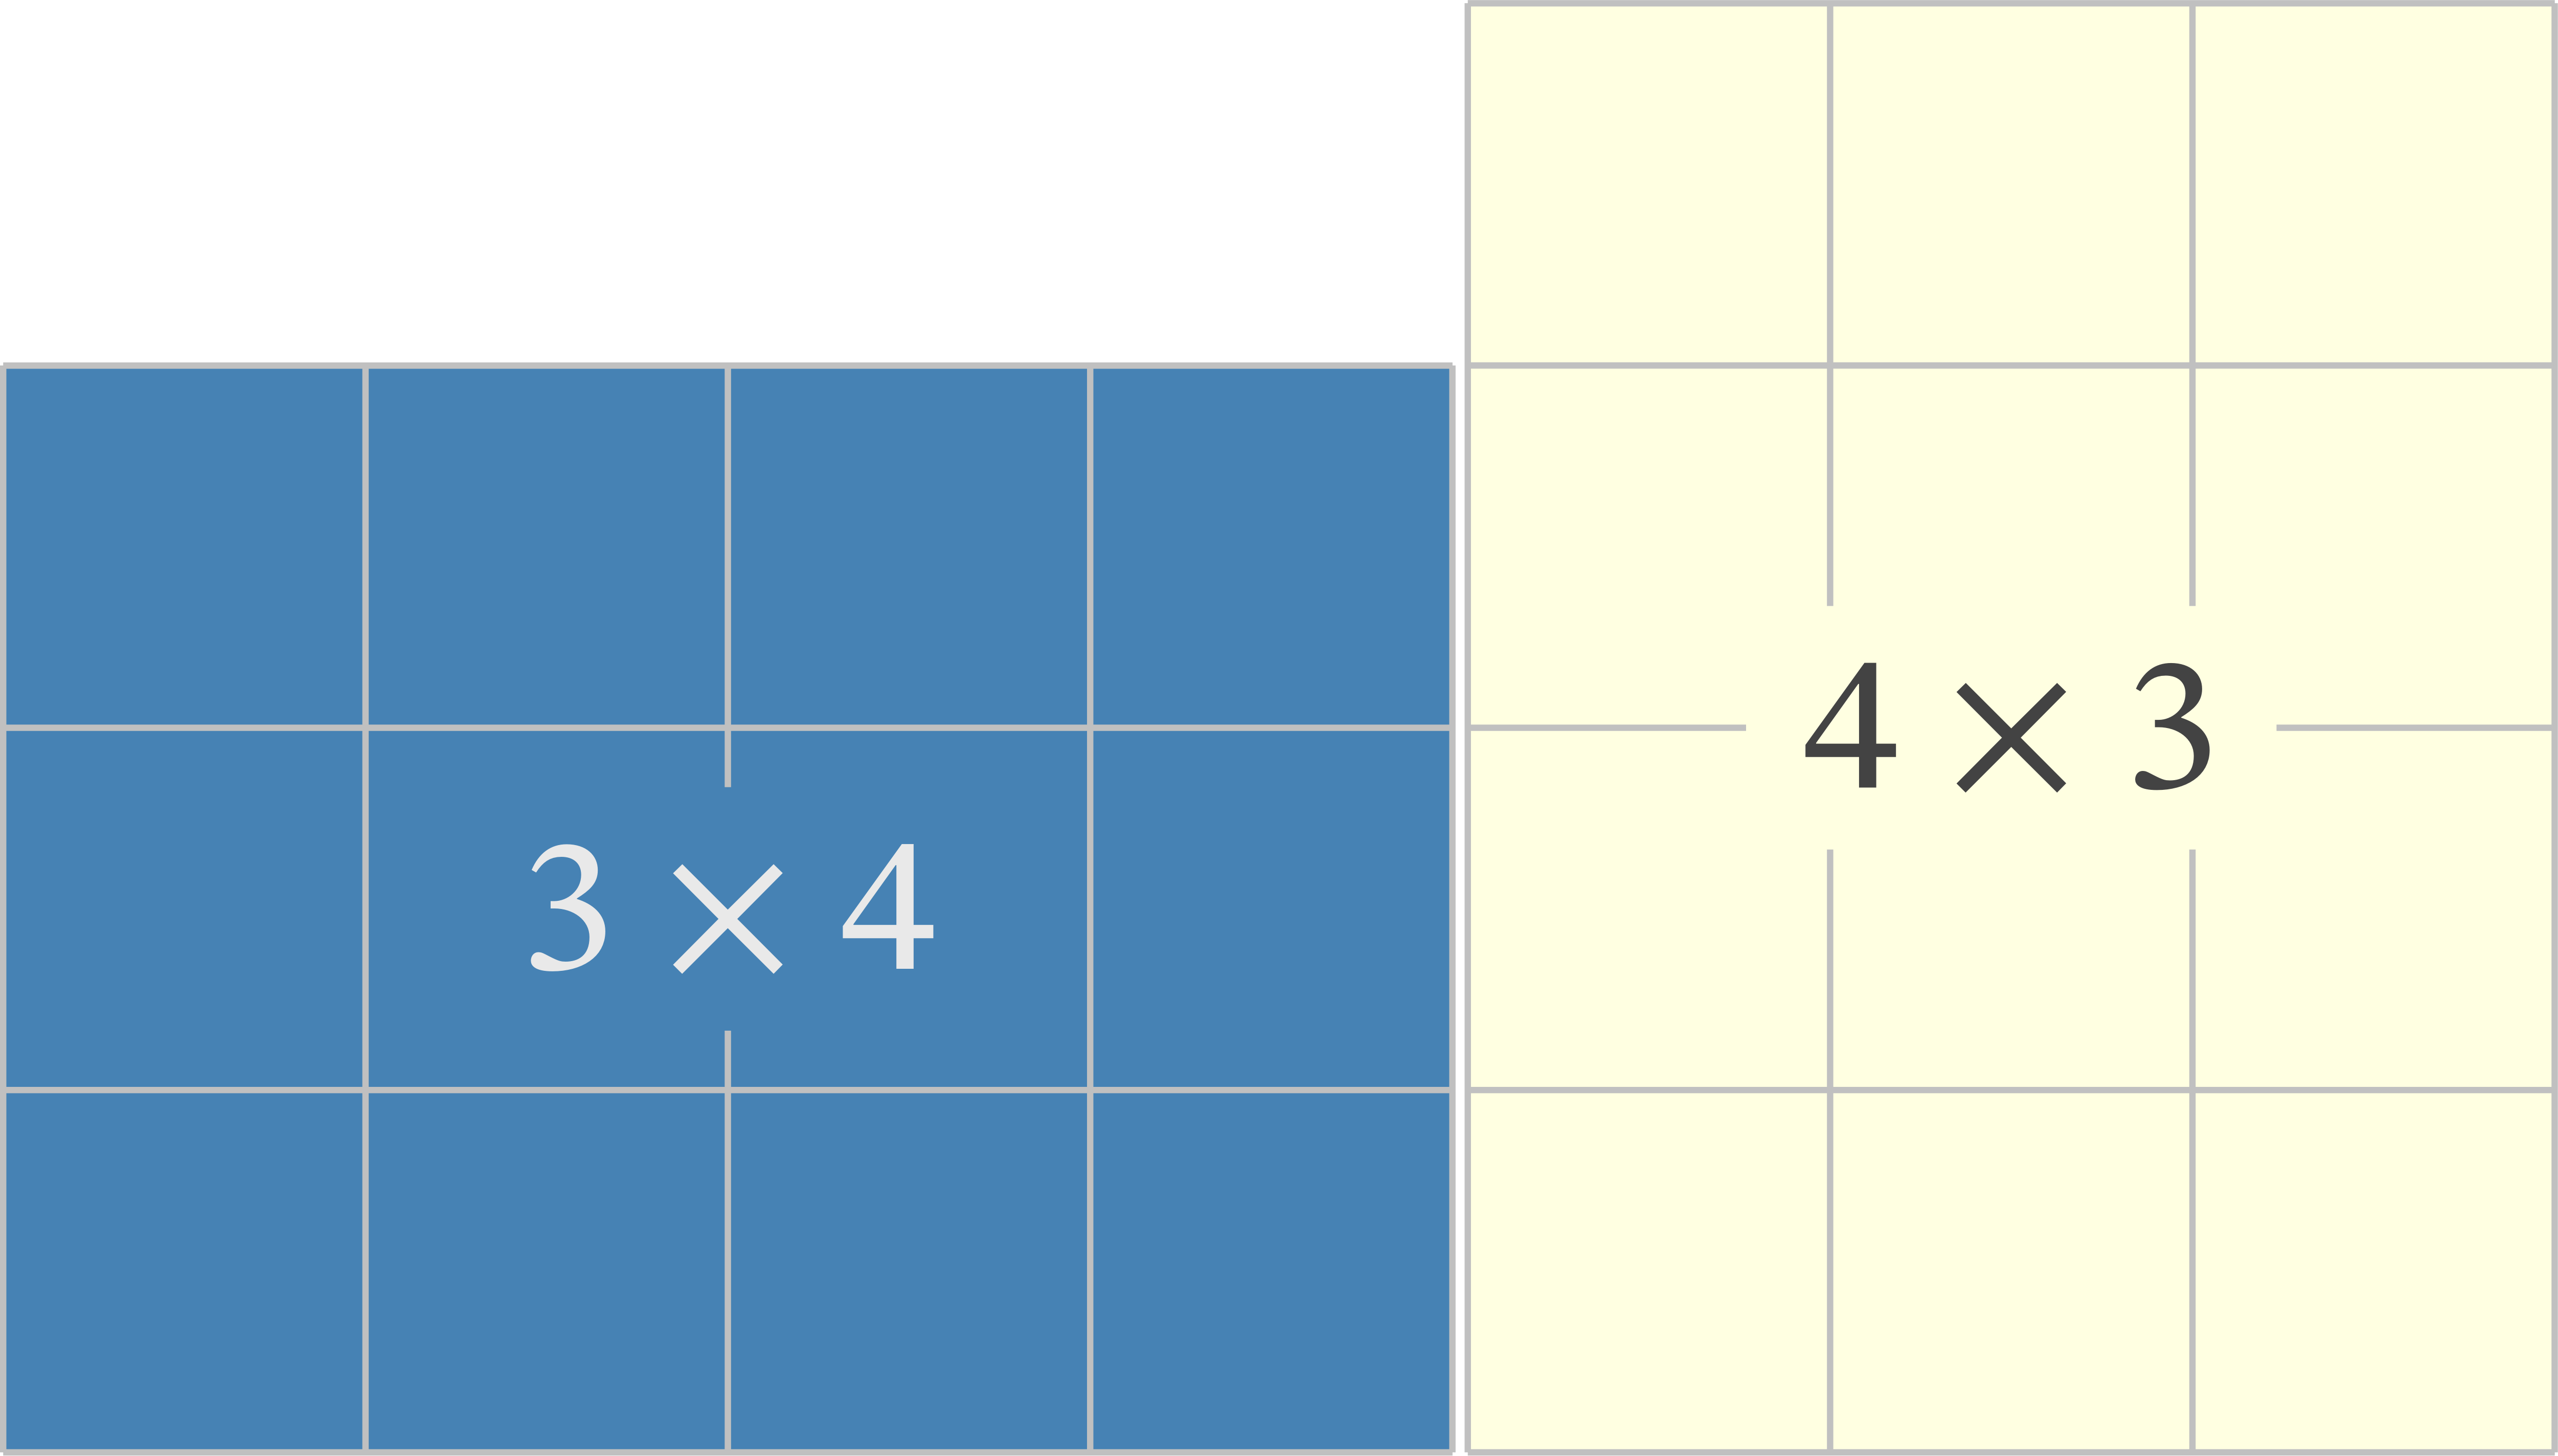
\includegraphics[width=0.6\textwidth,height=\textheight]{images/four-by-three.png}
\caption{The products \(4\times3\) and \(3\times4\) amount to repeated
additions and yield the same result of 12.}\label{fig:mult}
}
\end{figure}

Talking about commutativity and associativity might seem like overkill
for the addition and multiplication of real numbers. But, identifying
these properties is a useful insight, as the more sophisticated
mathematical objects we will encounter later may not obey either or both
properties.

\hypertarget{the-additive-and-multiplicative-identity-elements-in-mathbbr}{%
\subsection{\texorpdfstring{The additive and multiplicative identity
elements in
\(\mathbb{R}\)}{The additive and multiplicative identity elements in \textbackslash mathbb\{R\}}}\label{the-additive-and-multiplicative-identity-elements-in-mathbbr}}

When zero is added to any real number, \(a\), we get the original number
\(a\) back as the sum:
\begin{equation}\protect\hypertarget{eq:addident}{}{
a + 0 = 0 + a = a.
}\label{eq:addident}\end{equation} We call \(0\) the \emph{additive
identity} for \(\mathbb{R}\).

Likewise, when we multiply \(a\) by \(1\), the original number is
returned as the product:
\begin{equation}\protect\hypertarget{eq:multident}{}{
a \times 1 = 1 \times a = a
}\label{eq:multident}\end{equation} The number \(1\) is called the
\emph{multiplicative identity} in \(\mathbb{R}\).

Zero and one enjoy their
\href{https://dictionary.cambridge.org/dictionary/english/coign-of-vantage}{coign
of vantage} as the \emph{unique} additive and multiplicative identities
respectively for the real numbers in \(\mathbb{R}\). But are their roles
generalizable to cover a larger variety of mathematical objects?

Mathematics as a discipline tends to generalize and extend simple ideas
to increasing levels of complexity, while at the same time maintaining
consistency in definition and behaviour across these disparate domains.
The additive and multiplicative identities may be so generalized, where
applicable.

\hypertarget{varieties-of-additive-and-multiplicative-identity-elements}{%
\subsection{Varieties of additive and multiplicative identity
elements}\label{varieties-of-additive-and-multiplicative-identity-elements}}

The zero of the complex numbers is \(0 + i(0) = 0\) as well. And adding
it to any complex number returns the original complex number.

\href{https://mathworld.wolfram.com/Polynomial.html}{Polynomials} are
expressions like \(x^2 + 3x + 1\) where \(x\) is some real or complex
variable. The zero polynomial is simply the constant polynomial
\(P(x) = 0\), and adding it to any polynomial again gives us back the
original polynomial.

A \href{https://mathworld.wolfram.com/Matrix.html}{matrix} is a
rectangular array of numbers, treated as a single unit mathematically. I
facetiously call matrices \emph{numbers in teabags}. Operations on
matrices follow their own rules, but for addition, they are intuitively
apparent.

Let us consider an arbitrary \(2 \times 2\) \emph{square matrix} like
\(\begin{bmatrix}a & b\\c & d\end{bmatrix}\). It has two horizontal rows
and two vertical columns, and therefore 4 elements. The additive
identity for this matrix is a \(2 \times 2\) square matrix, all of whose
entries are zero:
\begin{equation}\protect\hypertarget{eq:addidmatrix}{}{
\begin{bmatrix}
a & b\\
c & d
\end{bmatrix}
+
\begin{bmatrix}
0 & 0\\
0 & 0
\end{bmatrix}
=
\begin{bmatrix}
a & b\\
c & d
\end{bmatrix}
=
\begin{bmatrix}
0 & 0\\
0 & 0
\end{bmatrix}
+
\begin{bmatrix}
a & b\\
c & d
\end{bmatrix}
}\label{eq:addidmatrix}\end{equation}

The matrix \(\begin{bmatrix}1 & 0\\0 & 1\end{bmatrix}\) is the
\emph{multiplicative identity} for matrix multiplication for
\(2 \times 2\) matrices.\footnote{The rules of matrix multiplication are
  a little involved and will not detain us here. The interested reader
  is referred to another blog of mine for details.} Note that its
elements are solely ones and zeroes, with ones on the principal-diagonal
from top left to bottom right.
\begin{equation}\protect\hypertarget{eq:matmultident}{}{
\begin{bmatrix}
a & b\\
c & d
\end{bmatrix}
\begin{bmatrix}
1 & 0\\
0 & 1
\end{bmatrix}
= %
\begin{bmatrix}
a & b\\
c & d
\end{bmatrix}
=
\begin{bmatrix}
1 & 0\\
0 & 1
\end{bmatrix}
\begin{bmatrix}
a & b\\
c & d
\end{bmatrix}
}\label{eq:matmultident}\end{equation}

This is a simple example of how the seed ideas of the additive and
multiplicative identities, sown far and wide, germinate into shoots that
are surprisingly similar to the original ones. The numbers \(0\) and
\(1\) do indeed rule the roost for the simple reason that the original
object remains unchanged under the respective operation. Obviously, the
identity matrices will change with the matrix sizes, but the principles
remain the same.

\hypertarget{the-additive-inverse-in-mathbbz-mathbbq-and-mathbbr}{%
\subsection{\texorpdfstring{The additive inverse in \(\mathbb{Z}\),
\(\mathbb{Q}\), and
\(\mathbb{R}\)}{The additive inverse in \textbackslash mathbb\{Z\}, \textbackslash mathbb\{Q\}, and \textbackslash mathbb\{R\}}}\label{the-additive-inverse-in-mathbbz-mathbbq-and-mathbbr}}

The negative integers arose from subtractions like \((3 - 5)\), whose
result was not a positive integer, and therefore lay outside the
confines of \(\mathbb{N}\). The negative numbers were introduced to
rectify this deficit. The sets \(\mathbb{Z}\) and \(\mathbb{R}\) both
contain negative numbers, and can therefore lay claim to an additive
inverse. Every integer or real number \(a\) has an \emph{additive
inverse}, \(a'\) such that: \[
a + a' = a' + a = 0.
\] Any guesses as to what \(a'\) is? It is the number \(a\) prefixed
with a negative sign and written as \(-a\), i.e., \(a' = -a\). It is
noteworthy, that when we subtract any real number from itself, we get
zero, by the property of the additive inverse:
\begin{equation}\protect\hypertarget{eq:addinv}{}{
a - a = a + (-a) = 0 = (-a) + a.
}\label{eq:addinv}\end{equation} If you have heard of
\href{https://www.symmetrymagazine.org/article/september-2008/antimatters-science-fiction-debut?language_content_entity=und}{matter
and antimatter annihilating each other in real life or Science Fiction}
{[}\protect\hyperlink{ref-antimatter2008}{1}{]}, you can metaphorically
think of \(a\) and \(-a\) as one such pair, giving rise not to energy,
but to zero.\emojifont {😉} \normalfont

\hypertarget{the-multiplicative-inverse-in-mathbbz-mathbbq-and-mathbbr}{%
\subsection{\texorpdfstring{The multiplicative inverse in
\(\mathbb{Z}\), \(\mathbb{Q}\), and
\(\mathbb{R}\)}{The multiplicative inverse in \textbackslash mathbb\{Z\}, \textbackslash mathbb\{Q\}, and \textbackslash mathbb\{R\}}}\label{the-multiplicative-inverse-in-mathbbz-mathbbq-and-mathbbr}}

Suppose we ask the question, ``If we have an arbitrary number \(a\),
what number should it be multiplied by to get \(1\)?'' Let us denote
this number by \(a''\). Then, we have:
\begin{equation}\protect\hypertarget{eq:multinv}{}{
a \times a'' = a'' \times a = 1
}\label{eq:multinv}\end{equation} If you know how to solve simple
equations, you would suggest that we divide \cref{eq:multinv} by \(a\)
on \emph{both sides}, like so:
\begin{equation}\protect\hypertarget{eq:solve}{}{
\begin{aligned}
a \times a'' &= 1; \mbox{ divide both sides by } a\\
a'' &= \frac{1}{a}.
\end{aligned}
}\label{eq:solve}\end{equation} The number \(\frac{1}{a}\) is called the
\emph{reciprocal} of \(a\) and it is the multiplicative inverse of
\(a\). But there is one important restriction: \(a \ne 0\). See
\protect\hyperlink{why-is-division-by-zero-disallowed}{Why is division
by zero disallowed?}

The rational numbers \(\mathbb{Q}\) arose to accommodate the results of
division. Note the hierarchy
\(\mathbb{N} \subset \mathbb{Z} \subset \mathbb{Q} \subset \mathbb{R}\)
where the symbol \(\subset\) may be spoken as ``is a subset of'' or ``is
contained in''.

\hypertarget{the-arithmetic-four-revisited}{%
\subsection{The Arithmetic Four
Revisited}\label{the-arithmetic-four-revisited}}

\hypertarget{addition}{%
\subsubsection{Addition}\label{addition}}

If we start with \(0\) and add \(1\) to it, we get \(1\). If we add
\(1\) to that we get \(2\). In this fashion, all the natural numbers may
be generated successively by adding \(1\). The \emph{next number} is
called the \emph{successor}. Even if we did not start with \(0\), but
started with \(1\) instead, we can still generate the entire set
\(\mathbb{N}\) by adding \(1\) successively.

This method shows that there is no largest natural number. If there were
such a number, say \(p\), we could always add one to it and show the
assumption to be false, since \((p + 1) > p\). In this sense, the number
\(1\) helps us to understand
\href{https://mathinsight.org/definition/countably_infinite}{countable
infinity}.

\hypertarget{subtraction}{%
\subsubsection{Subtraction}\label{subtraction}}

Subtracting zero from a number leaves it unchanged: \(a - 0 = a\).

By convention, when a sign is not prefixed to a number, we assume it to
be positive. If a negative sign is prefixed to a number, it is a
negative number. This is indicated by a pair of
parentheses---surrounding the number and its sign---in expressions. When
the number is featured alone, these parentheses are dropped.

With signed numbers, from \(\mathbb{Z}\), \(\mathbb{Q}\), or
\(\mathbb{R}\), we may convert any subtraction into an addition thus:
\begin{equation}\protect\hypertarget{eq:negnum}{}{
3 - 5 = -2 = 3 + (-5) = (-5) + 3.
}\label{eq:negnum}\end{equation} And those additions would still be
commutative. This does not mean that subtraction has suddenly become
commutative; it has not. It simply means that subtraction can be morphed
into the (commutative) addition of signed numbers.

\hypertarget{multiplication}{%
\subsubsection{Multiplication}\label{multiplication}}

Multiplying any number \(a\) by zero yields zero:
\(a \times 0 = 0 \times a = 0\). This might be a little difficult to
grasp. To see why this is the case, let us be a little sneaky and write
zero as \((p + (-p))\), for some \(p \in \mathbb{R}\), because \[
(p + (-p)) = p - p = 0.
\] Then, we may write, for arbitrary \(a \in \mathbb{R}\),
\begin{equation}\protect\hypertarget{eq:multzero}{}{
\begin{aligned}
a \times 0 &= a \times (p + (-p))\\
&= a \times p + a\times (-p)\\
&= ap - ap\\
&= 0.
\end{aligned}
}\label{eq:multzero}\end{equation} Here, I have invoked the rule that
the product of a positive and a negative number is negative.

Zero was a problematic number that had been introduced into Europe from
India via the Arabs. Can you imagine the effort that must have gone into
understanding and justifying that multiplication of any number by zero
yielded zero? Zero, one, and infinity are a daunting triad. Mastering
them takes time, practice, and familiarity, and stretches both human
logic and imagination.

Multiplying a number by \(1\) is comparatively simpler: it leaves the
original number unchanged. The number \(1\) is the \emph{multiplicative
identity} element for the real numbers. So,
\(5 \times 1 = 1 \times 5 = 5\).

Multiplying \(a\) by \(-1\) yields the additive inverse of \(a\), namely
\(-a\).

\hypertarget{division}{%
\subsubsection{Division}\label{division}}

If multiplication can be thought of as repeated addition, division can
equally be thought of as repeated subtraction. Dividing \(6\) by \(2\)
may be understood as ``How many times can we subtract \(2\) from \(6\)
before we hit zero?'' Stated a little more mathematically,
\(6 \div 2 = 3\), and the steps are: \[
\begin{array}{r | l}
6 - 2 = 4 & \mbox{First lot of two}\\
4 - 2 = 2 & \mbox{Second lot of two}\\
2 - 2 = 0 & \mbox{Third lot of two}\\
\end{array}
\] The result or \emph{quotient} is \(3\) because our subtraction
algorithm terminated in \(3\) steps with a remainder of \(0\). Because
division is the inverse of multiplication, we can also understand the
result as the number by which we must multiply the \emph{divisor} \(2\)
to obtain the \emph{dividend} \(6\). In this case, the \emph{remainder}
is zero, to better illustrate what is happening.

If the division gives rise to a remainder, we stop when we get a
remainder that is less than the divisor. For example, with \(7 \div 2\),
we get: \[
\begin{array}{r | l}
7 - 2 = 5 & \mbox{First lot of two}\\
5 - 2 = 3 & \mbox{Second lot of two}\\
3 - 2 = 1 & \mbox{Third lot of two}\\
\end{array}
\] That last number \(1\) is the remainder and the number of steps
before stopping is still the quotient, which is again \(3\).

Just as subtraction may be thought of as addition of signed numbers, so
also, division may be thought of as multiplication by reciprocals. If
some real \(a\) is divided by another real \(b \ne 0\), we may write
this as \(a \div b\) or equivalently, we may also express it as
\(a \times \frac{1}{b} = \frac{1}{b} \times a = \frac{a}{b}\).

\hypertarget{why-is-division-by-zero-disallowed}{%
\subsubsection{Why is division by zero
disallowed?}\label{why-is-division-by-zero-disallowed}}

Now, what happens if we divide by zero? To keep matters simple, let us
keep the same dividend, namely 6. If we subtract 0 from 6, we end up
with 6. Subtracting another 0 from this 6 still leaves us with 6. By
now, you should have cottoned on to the fact that we are not making any
progress. \[
\begin{array}{r | l}
6 - 0 = 6 & \mbox{First lot of zero}\\
6 - 0 = 6 & \mbox{Second lot of zero}\\
6 - 0 = 6 & \mbox{Third lot of zero}\\
\cdots & \cdots\\
\end{array}
\] Each time we subtract zero, the remainder equals the dividend, and we
end up where we started. Thus, this process never ends, and therefore
cannot be an
\href{https://mathworld.wolfram.com/Algorithm.html}{algorithm}, which by
definition, must terminate in a \emph{finite} number of steps.
Sometimes, this is stated as ``dividing by zero gives infinity,'' which
is a mathematically less acceptable, but intuitively more friendly, way
of stating that it is an unending process. This is why division by zero
is not permitted.

The most basic justification for not permitting division by zero is
given here. With increasing mathematical sophistication, increasingly
recondite reasoning may be given for why division by zero is not
permitted. For example, \emph{any number} multiplied by zero gives zero.
Therefore, dividing by zero will give us \emph{any number}, which is a
non-unique answer. Allowing such an operation will destroy the
predictability on which mathematical operations are built.

\hypertarget{exponentiation}{%
\subsection{Exponentiation}\label{exponentiation}}

Exponentiation may also be called \emph{raising (something) to a power}.
It is a short form for repeated multiplication by the \emph{same}
number. For example, if we multiply \(5\) by itself three times, we
write it so: \begin{equation}\protect\hypertarget{eq:exp}{}{
5\times5\times5 = 5^1\times5^1\times5^1 = 5^{(1+1+1)} = 5^{3} = 125
}\label{eq:exp}\end{equation} The number \(5\) is called the \emph{base}
and the power \(3\) is called the \emph{exponent}. Note that \(5^1 = 5\)
and the exponent \(1\) is omitted.

The reciprocal of an arbitrary non-zero real number \(a\) is
\(\frac{1}{a}\). The product of the two is \(1\). Written with an
exponent, \[
\frac{1}{a} = a^{-1}.
\] Continuing with the number \(5\) in our example, its reciprocal is
\(\frac{1}{5} = 5^{-1}\). What do we get if we multiply \(5\) by its
reciprocal? We already know the answer to be \(1\). Let us do the
multiplication using exponents:
\begin{equation}\protect\hypertarget{eq:reciprocal}{}{
5 \times \frac{1}{5} = 1 = 5^{1} \times 5^{-1} = 5^{1+(-1)} = 5^{0}.
}\label{eq:reciprocal}\end{equation} The astounding conclusion from
\cref{eq:reciprocal} is that \(5\) raised to the exponent zero is
\({1}\). I will hand-wave here and assert that this will apply to any
base \(a \in \mathbb{R}\), i.e., \(a^0 = 1\) for \(a \in \mathbb{R}\):
something that will be understood better after we encounter
\href{https://www.britannica.com/science/logarithm}{logarithms} in this
series of blogs or elsewhere. The consequence is that the logarithm of
\(1\) to any base \(b\) is \(0\):
\begin{equation}\protect\hypertarget{eq:logonezero}{}{
log_{b}1 = 0.
}\label{eq:logonezero}\end{equation} \cref{eq:logonezero} is yet another
memorable equation linking \(1\) and \(0\). When the domain of
mathematics expands to take on new numbers, new objects, and new
notations, the need for consistency with the existing body of
mathematics gives us pearls such as equation \cref{eq:logonezero}.

From the foregoing, note that \[
a \times \frac{1}{a} = a \times a^{-1} = a^0 = 1.
\]

Constants in polynomials may be written using \(x^0\) in place of one.
Fir example, \begin{equation}\protect\hypertarget{eq:polyexp}{}{
2x^2 + 3x + 2 = 2x^2 + 3x^1 + 2x^0.
}\label{eq:polyexp}\end{equation} \cref{eq:polyexp} show how
consistently the terms in a polynomial are: they are all powers of \(x\)
in descending fashion, although by convention, certain terms are
understood and therefore implicit. The omission of the index in the term
\(3x^1\) and the term \(x^0\) could cause disquiet in the newcomer to
polynomials, and it is better to dispel that right away.

In the succeeding sections, we take a look a some lesser known aspects
of zero and one.

\hypertarget{the-shy-one}{%
\subsection{The shy one}\label{the-shy-one}}

The number one is often
\href{https://www.vocabulary.com/dictionary/implicit}{implicit} in
mathematical notation. While we may write \(2x\) to denote
\(2\times x\), or two multiplied by \(x\), we \emph{do not} write
\(1x\), even if it is literally correct, because of convention. In
instances like this, the number one is implicit, and assumed to be
understood by those who know. If you happen to be one of those
\emph{not} in the know, here's your chance to join the other side.

When we write a fraction as \(\frac{3}{4}\) we mean the decimal \(0.75\)
and matters are clear. But all whole numbers are also fractions with the
denominator being \(1\). So, the fraction \(\frac{3}{1}\) is rarely
written in that form, even if syntactically correct, because usage
dictates that whole numbers are written to stand on their own, as \(3\),
in this case. Again, the \(1\) in the denominator is assumed to be
unobtrusively present:
\href{https://dictionary.cambridge.org/dictionary/english/out-of-sight-out-of-mind}{out
of sight but \emph{not} out of mind}.

When we write \(4^2\), spoken out as ``four squared'' we mean the number
obtained by multiplying \(4\) by itself. This nomenclature arose
because, if 4 was associated with the \emph{length} of, say, a piece of
string, the number ``four squared'' was used to denote the \emph{area}
of a square that had a side of length \(4\). So,
\(4^2 = 4\times4 = 16\).

Likewise, the expression \(7^3\) or ``seven cubed'' denoted the volume
of a cube of side \(7\). Beyond the third dimension, this naming scheme
faded out, because we cannot percieve dimensions higher than three.

Therefore, \(6^4\) is spoken as ``six raised to the fourth (power)'' or
``six to the four''. In such statements, the number \(6\) is called the
\emph{base} and the number \(4\) is called the \emph{exponent}.

Following this logic, we might assert that \(5^1 = 5\) and that is
perfectly correct. But again, convention intrudes to say that we write
it simply as \(5\). \emph{Any number raised to the power of \(1\) equals
itself}.

The notation making \(1\) implicit in these scenarios reduces clutter
and simplifies notation. The absence of the implicit \(1\) might trouble
the heart of the sincere young mathematician, but familiarity with these
conventions will make for comfort in using them.

\hypertarget{the-interval-0-1}{%
\subsection{\texorpdfstring{The interval
\([0, 1]\)}{The interval {[}0, 1{]}}}\label{the-interval-0-1}}

If the reals are thought of as a line, the segment from \(0\) to \(1\)
can serve as a microcosm of all the real numbers. It is as densely
populated with rational and irrational numbers as the entire real number
line. This almost holographic property is a consequence of what
``infinity'' is, and is again a concept that might be difficult to
accept, let alone understand.

In any case, our interest in the
\href{https://mathworld.wolfram.com/ClosedInterval.html}{closed
interval} \([0, 1]\) is for a different purpose now. The numbers in
\(\mathbb{Q}\) and \(\mathbb{R}\) have an interesting property when they
lie in the interval \([0, 1]\). If we raise such numbers to integer
powers, they become progressively smaller in value. This may easily be
seen using the rules of exponentiation, or by successive multiplication.

Let \(a = 0.9\). Then we may tabulate successive integral powers of as
tabulated below. \[
\begin{array}{l | r | l}
a & 0.9^1 & 0.9\\
a^2 & 0.9^2 & 0.81\\
a^3 & 0.9^3 & 0.729\\
a^4 & 0.9^4 & 0.6561\\
a^5 & 0.9^5 & 0.59049\\
\end{array}
\] It is clear that the powers of \(a^n\) diminish with increasing \(n\)
when \(a \in [0, 1]\).This is peculiar to the interval \([0, 1]\),
because when \(a > 1\), the powers of \(a^n\) increase with increasing
\(n\), as tabulated below for \(a=1.1\). \[
\begin{array}{l | r | l}
a & 1.1^1 & 1.1\\
a^2 & 1.1^2 & 1.21\\
a^3 & 1.1^3 & 1.331\\
a^4 & 1.1^4 & 1.4641\\
a^5 & 1.1^5 & 1.61051\\
\end{array}
\] The pivot at \(a = 1\) is rock steady because \(1^n = 1\) for all
\(n \in \mathbb{N}\). When \(a\) is 10\% less, we see a steady decline
in \(a^n\) as \(n\) increases. But when \(a\) is 10\% more than \(1\),
we see a growth in \(a^n\) and \(n\) increases. This wondrous behaviour
contributes to the magic of the number \(1\).

\cref{fig:x-to-n} shows graphs of \(x^n\) for \(x \in [0, 1]\) and
\(n = 0, 1, 2, 4, 8, 128, 512\). As \(n\) increases and \(x\) approaches
\(1\), the graphs exhibit an almost perpendicular change in direction
like a laterally inverted \(L\). I find this behavior fascinating.

\begin{figure}
\hypertarget{fig:x-to-n}{%
\centering
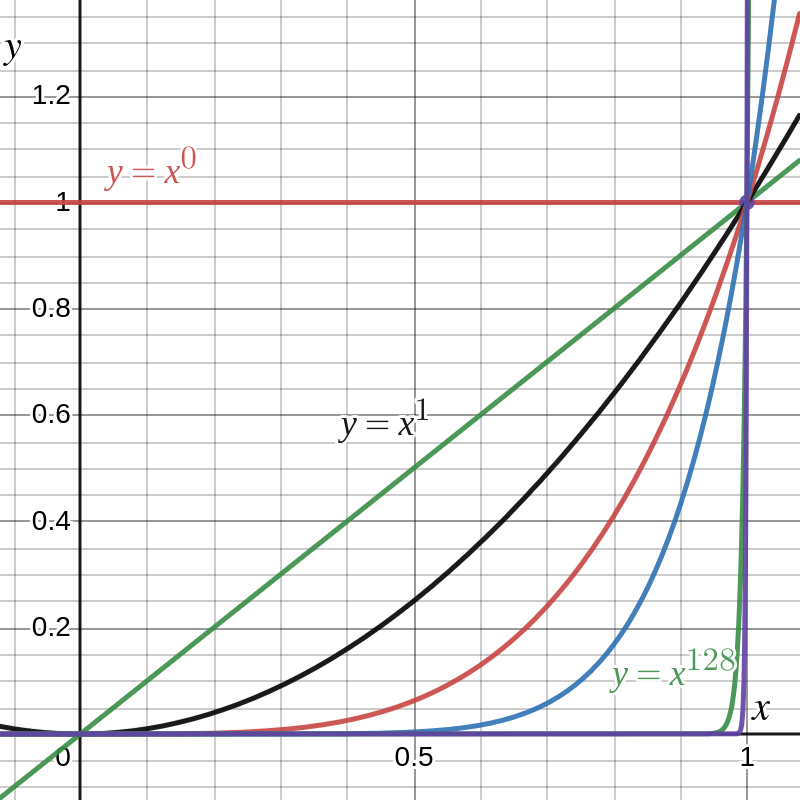
\includegraphics[width=0.7\textwidth,height=\textheight]{images/y-equals-x-to-the-n-in-0-1.png}
\caption{Graphs of \(y = x^n\) for \(x \in [0, 1]\) and
\(n = 0, 1, 2, 4, 8, 128, 512\). Note that all curves pass through
\((1, 1)\).}\label{fig:x-to-n}
}
\end{figure}

\hypertarget{rotation-on-the-complex-plane}{%
\subsection{Rotation on the complex
plane}\label{rotation-on-the-complex-plane}}

The two-dimensional plane may be pressed into service in a variety of
contexts to serve different ends. One such use is the
\href{https://mathworld.wolfram.com/ArgandDiagram.html}{Argand diagram}
in which the \(x\) axis represents the real part and the \(y\) axis the
imaginary part of a complex number,
\(z = x + iy; x, y \in \mathbb{R}; z \in \mathbb{C}\).

\hypertarget{binary-logic-and-numbers}{%
\subsection{Binary logic and numbers}\label{binary-logic-and-numbers}}

\hypertarget{sequences}{%
\subsection{Sequences}\label{sequences}}

An ordered procession of numbers is called
\href{https://en.wikipedia.org/w/index.php?title=Sequence\&oldid=1177801065}{sequence}
{[}\protect\hyperlink{ref-wikisequence}{2},\protect\hyperlink{ref-wolframsequence}{3}{]}.\footnote{The
  general definition replaces \emph{numbers} with \emph{mathematical
  objects} but the former will suffice for our limited purpose here.}
Repetitions are allowed, but the order matters. The natural numbers form
the sequence \((1, 2, 3, 4, 5, \ldots)\). Note that the elements of the
sequence are enclosed in parentheses, \(()\). There is an entire website
devoted to sequences, called the \href{https://oeis.org/}{The On-Line
Encyclopedia of Integer Sequences® (OEIS®)}.

Fibonacci sequence

Binomial sequence Pascals triangle

\hypertarget{series}{%
\subsection{Series}\label{series}}

A \href{https://mathworld.wolfram.com/Series.html}{series} is the
(progressive) sum of an infinite sequence
{[}\protect\hyperlink{ref-wikiseries}{4},\protect\hyperlink{ref-wolframseries}{5}{]}.

Pascal's triangle and the Binomial theorem and their origin in the
number 1.

Arithmetic series (progressions)

Geometric series (progressions)

https://en.wikipedia.org/wiki/Circle\_group

Circle Circle\_group

\hypertarget{acknowledgements}{%
\subsection{Acknowledgements}\label{acknowledgements}}

\hypertarget{feedback}{%
\subsection{Feedback}\label{feedback}}

Please \href{mailto:feedback.swanlotus@gmail.com}{email me} your
comments and corrections.

\noindent A PDF version of this article is
\href{./the-two-most-important-numbers.pdf}{available for download
here}:

\begin{small}

\begin{sffamily}

\url{https://swanlotus.netlify.app/blogs/the-two-most-important-numbers.pdf}

\end{sffamily}

\end{small}

\hypertarget{bibliography}{%
\section*{References}\label{bibliography}}
\addcontentsline{toc}{section}{References}

\hypertarget{refs}{}
\begin{CSLReferences}{0}{0}
\leavevmode\vadjust pre{\hypertarget{ref-antimatter2008}{}}%
\CSLLeftMargin{{[}1{]} }%
\CSLRightInline{William S Higgins. 2008. {Antimatter's science fiction
debut}. Retrieved 5 November 2023 from
\url{https://www.symmetrymagazine.org/article/september-2008/antimatters-science-fiction-debut?language_content_entity=und}}

\leavevmode\vadjust pre{\hypertarget{ref-wikisequence}{}}%
\CSLLeftMargin{{[}2{]} }%
\CSLRightInline{Wikipedia contributors. 2023. {Sequence---{Wikipedia}{,}
The Free Encyclopedia}. Retrieved 3 November 2023 from
\url{https://en.wikipedia.org/w/index.php?title=Sequence\&oldid=1177801065}}

\leavevmode\vadjust pre{\hypertarget{ref-wolframsequence}{}}%
\CSLLeftMargin{{[}3{]} }%
\CSLRightInline{Eric W Weisstein. {Sequence. From MathWorld---A Wolfram
Web Resource}. Retrieved 3 November 2023 from
\url{https://mathworld.wolfram.com/Sequence.html}}

\leavevmode\vadjust pre{\hypertarget{ref-wikiseries}{}}%
\CSLLeftMargin{{[}4{]} }%
\CSLRightInline{Wikipedia contributors. 2023. {Series
(mathematics)---{Wikipedia}{,} The Free Encyclopedia}. Retrieved 3
November 2023 from
\url{https://en.wikipedia.org/w/index.php?title=Series_(mathematics)\&oldid=1174621451}}

\leavevmode\vadjust pre{\hypertarget{ref-wolframseries}{}}%
\CSLLeftMargin{{[}5{]} }%
\CSLRightInline{Eric W. Weisstein. {Series. From MathWorld---A Wolfram
Web Resource}. Retrieved 3 November 2023 from
\url{https://mathworld.wolfram.com/Series.html}}

\end{CSLReferences}



\end{document}
